\documentclass[10pt]{article}
\usepackage[utf8]{inputenc}
\usepackage{graphicx}
\usepackage[export]{adjustbox}
\graphicspath{ {docs/latex/images/} }

\title{Rapport Projet GL}
\date{}
\author{}

\begin{document}
\large
\begin{titlepage}
    \centering
    \begin{minipage}{0.5\textwidth}

        \centering
        
\includegraphics[width=0.9\linewidth]{ensimag_logo.png}

        % Caption and label can be added here if desired
    \end{minipage}%

    
    {\scshape\LARGE Grenoble INP-ENSIMAG  \par}
    \vspace{4cm}
    {\scshape\Large  Conception :  jeu de simulation boursière \par}
    \vspace{8cm}
    {\Large\itshape CHRIF M'HAMED Mohamedou, EL IDRISSI Khaoula, MOHAMED AHMED Mohamed Lemine
\par}


\end{titlepage}

% pour sommaire :
\tableofcontents

%  page d'introduction :
\newpage
\section{\textbf{Introduction}}

Dans ce document, on explique la conception détaillée de la partie implémentée du cahier des charges. 
nous avons choisi d'implémenter une partie  important du chaier de charges comme l'achat et la vente d'actions, la simulation du prix d'une action avec interface graphique simple.



\section{\textbf{choix de l'Architecture : MVC}}

Pour implémenter ce jeu de simulation, nous avons adopté l'architecture MVC (Modèle - Vue - Contrôleur), avec une partie Modèle responsable de toute la logique liée à la gestion du portefeuille, à l'utilisateur ainsi qu'à l'achat et à la vente des actions.

La partie Vue concerne l'interface utilisateur, telle que le tableau de bord, etc., détaillée dans la section 4 de ce document. Enfin, la dernière partie, le Contrôleur, assure la communication entre la partie Vue et le Modèle

\newpage
\begin{figure}
 
    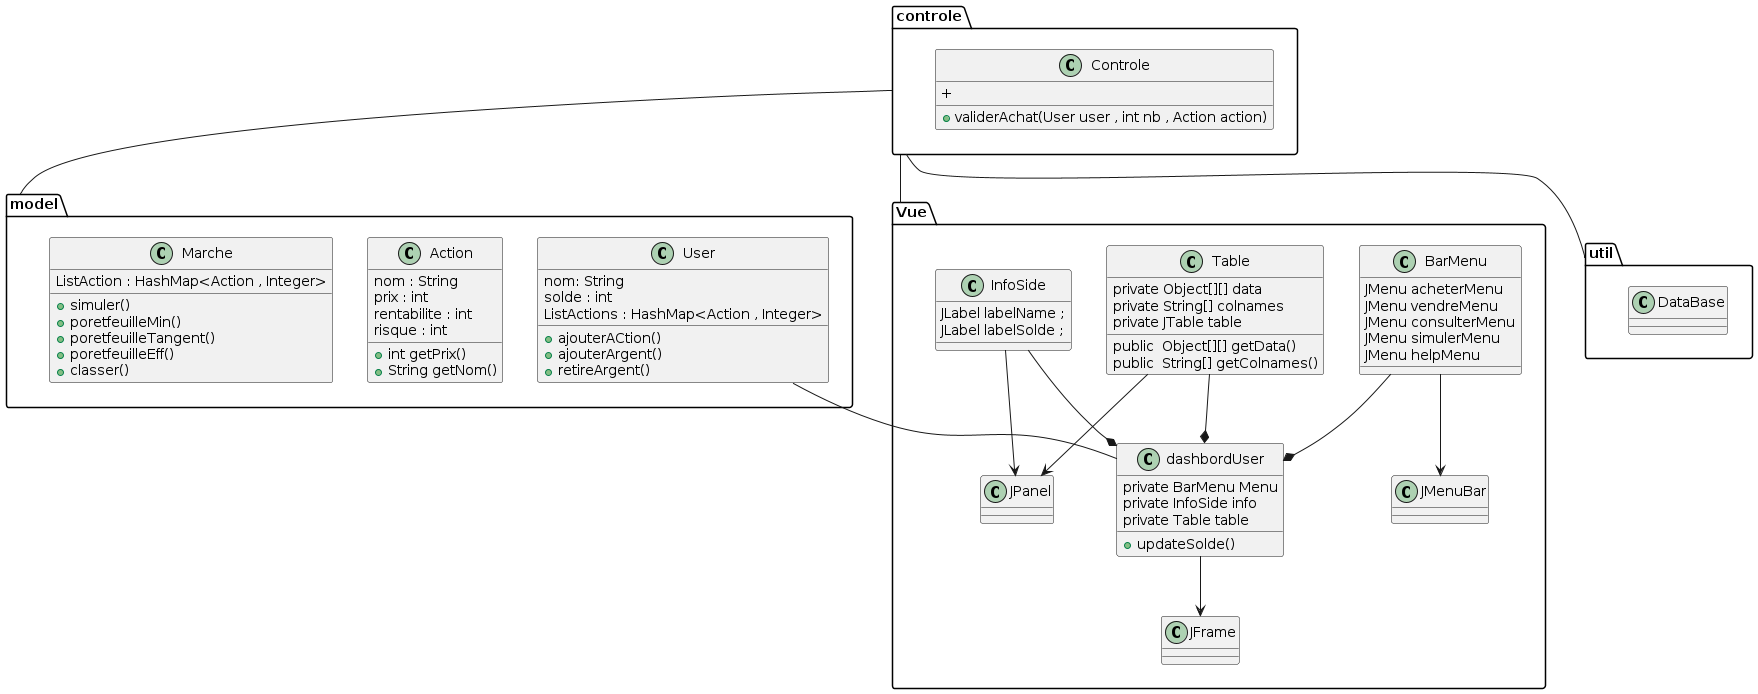
\includegraphics[height=0.5\textwidth]{Model.png}
    \caption{Conception MVC}
    \label{fig:enter-label}
\end{figure}

% page conception détaille :
\newpage
\section{\textbf{Conception du Modèle}}


Dans la conception du modèle, nous avons trois classes principales dans un package appelée: \textbf{modele}

\subsection{User}

\begin{itemize}
    \item  cette classe liée à toutes les opérations et les propriétes liée à l'utilisateur comme son nom et son solde

    \item  la classe \textbf{User} Présente une méthode essentielle
    \newline
    \textbf{ajouterAction(Action choix , int nb)} qui  est appelée lors de l'achat d'une action pour valider que l'utilisateur dispose d'un solde suffisant pour cet achat.
    
    \item  Pour  les actions de l'utilisateur, nous stockons celles-ci dans une \textbf{HashMap} afin de réduire la complexité de la recherche de \textbf{$\Theta(n)$} à \textbf{$\Theta(1)$}.

\end{itemize}

\begin{figure}
    \centering
    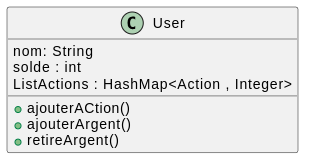
\includegraphics[width=0.5\linewidth]{User.png}
    \caption{User}
    \label{fig:enter-label}
\end{figure}


\subsection{Marche}

\begin{itemize}
    \item Cette classe est liée à toutes les opérations concernant le marché lui-même, telles que l'ajout d'actions particulières ou l'attribution des actions à un utilisateur lors de l'achat
    
    \item Pour les actions du marché , nous générons des actions aléatoires pour les prix suivant une loi uniforme continue entre 100 et 400, et pour les rentabilités et les risques suivant une loi normale centrée réduite.

\end{itemize}

\begin{figure}
    \centering
    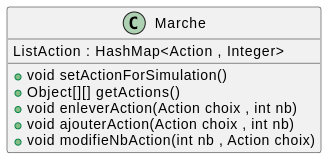
\includegraphics[width=0.5\linewidth]{Marche.png}
    \caption{Marche}
    \label{fig:enter-label}
\end{figure}


\subsection{Action}
\begin{itemize}
    \item  cette classe réprsente une action dans le marché finaiciére 

    \item chaque action est carcatériser par : nom , prix , rentabilité , risque 
\end{itemize}

\begin{figure}
    \centering
    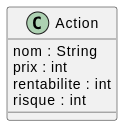
\includegraphics[width=0.25\linewidth]{action.png}
    \caption{Action}
    \label{fig:enter-label}
\end{figure}



% paage conception de l'interface utilisateur  :
\newpage
\section{\textbf{Conception de l'interface utilisateur}}

Nous avons tenté de concevoir une interface utilisateur conviviale en utilisant le package \textbf{java.swing}, en intégrant des dépendances externes telles que \textbf{JFreeChart} pour simuler des actions . \\
\newline
Dans cette section, nous expliquons brièvement la hiérarchie de classes que nous avons utilisée pour implémenter l'interface utilisateur \\

\begin{figure}
 
    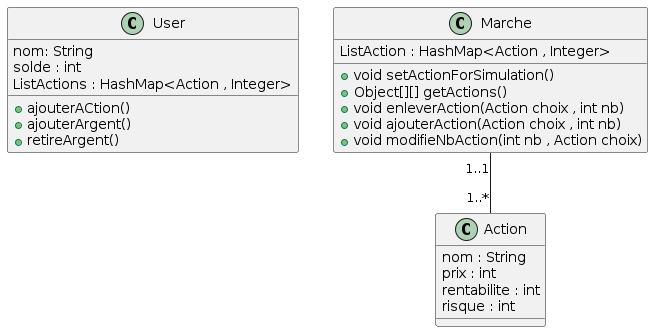
\includegraphics[height=0.5\textwidth]{model_conception.png}
    \caption{Conception Modele}
    \label{fig:enter-label}
\end{figure}





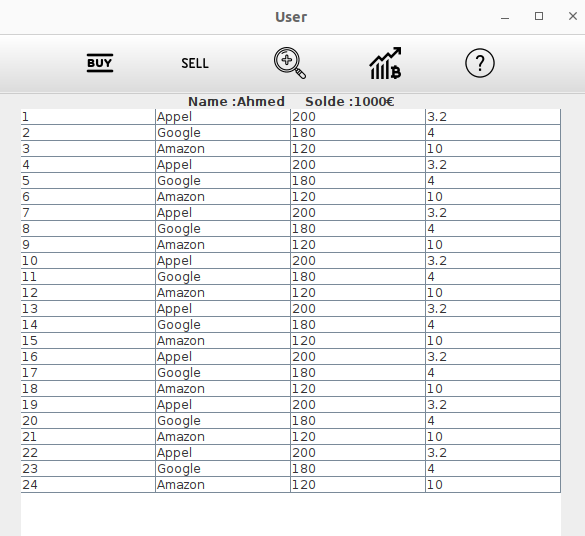
\includegraphics[width=0.9\linewidth]{user_interface.png}
\newline





\begin{itemize}
    \item \textbf{class dashbordUser} : Cette classe est la classe principale de l'interface graphique. Elle contient 3 attributs : un attribut représentant la table des actions du client, le BarMenu qui contient les fonctionnalités de l'application, et un attribut 'info' qui contient des informations personnelles telles que le nom et le solde."

    \item \textbf{class BarMenu}
        Cette classe contient toutes les fonctionnalités de l'application, telles que l'achat/la vente d'actions ou la simulation du marché financier.

    \item \textbf{InfoSide} 
        Cette classe contient les informations personnelles du client, telles que son nom et son solde.

    \item \textbf{Table}
        La classe Table est responsable de la partie vue de la table des actions de l'utilisateur.
    
\end{itemize}


\begin{figure}
    \centering
    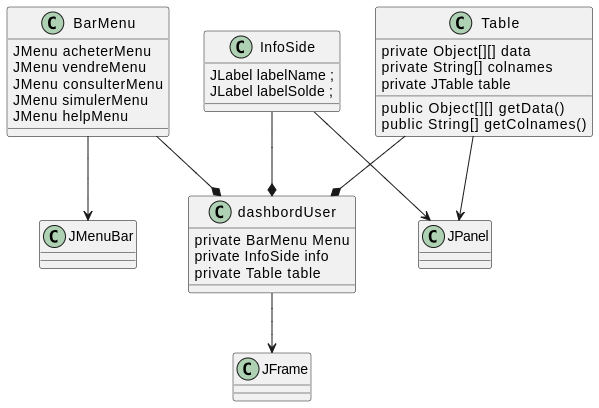
\includegraphics[width=1\linewidth]{GUI.png}
    \caption{Conception de l'interface utilisateur}
    \label{fig:enter-label}
\end{figure}



% \subsection{Conception du BarMenu}

% Si l'utilisateur clique sur le bouton 'acheter', par exemple, dans la classe BarMenu, un MouseListener détecte le clic sur le bouton 'acheter' et instancie la classe 'Acheter' .\\
%  \newline 
% \textbf{Diagramme de séquence:}






\end{document}
